\documentclass[a4paper,12pt]{article}
\usepackage{fontspec}
\setmainfont{Times New Roman}
\setmonofont{DejaVu Sans Mono}[Scale=0.85]
\usepackage[top=3cm,bottom=3.5cm,left=3.5cm,right=2cm]{geometry}
\usepackage{setspace,amsmath,unicode-math,array,booktabs,tabularx,longtable,enumitem,tikz,xurl}
\setmathfont{Latin Modern Math}
\usetikzlibrary{arrows.meta,positioning}
\usepackage{titlesec,caption,cite}
\usepackage[unicode,hidelinks]{hyperref}
\hypersetup{pdftitle={N01 M1 - Báo cáo khảo sát và đề xuất giải pháp},pdfauthor={Phan Chí Kiên; Hồ Nhật Khanh}}
\makeatletter
\renewcommand\normalsize{\@setfontsize\normalsize{13}{16}}
\makeatother
\AtBeginDocument{\normalsize\onehalfspacing}
\renewcommand{\refname}{Tài liệu tham khảo}
\renewcommand{\tablename}{Bảng}
\renewcommand{\figurename}{Hình}
\titleformat{\section}{\normalsize\bfseries}{\thesection.}{0.5em}{}
\titleformat{\subsection}{\normalsize\bfseries}{\thesubsection.}{0.5em}{}
\titlespacing*{\section}{0pt}{9pt}{3pt}
\titlespacing*{\subsection}{0pt}{6pt}{2pt}
\setlength{\parindent}{1cm}
\setlength{\parskip}{0pt}
\setlength{\emergencystretch}{3em}
\setlength{\tabcolsep}{4pt}
\setlist{nosep,leftmargin=1.5em}
\captionsetup{font=normalsize,labelfont=bf,labelsep=colon,hypcap=false}
\newcolumntype{L}[1]{>{\raggedright\arraybackslash}p{#1}}
\newcolumntype{Y}{>{\raggedright\arraybackslash}X}
\newcommand{\code}[1]{\texttt{#1}}
\newcommand{\tblfont}{\setstretch{1.0}\normalsize}
\begin{document}
\hypersetup{pageanchor=false}
\begin{titlepage}
\centering
\textbf{ĐẠI HỌC QUỐC GIA THÀNH PHỐ HỒ CHÍ MINH}\\
\textbf{TRƯỜNG ĐẠI HỌC CÔNG NGHỆ THÔNG TIN}\\
\textbf{KHOA KỸ THUẬT MÁY TÍNH}
\vspace{2.0cm}

\textbf{ĐỒ ÁN 1 (CE201)}\\
\textbf{HK1 NĂM HỌC 2026--2027}
\vspace{1.2cm}

\textbf{BÁO CÁO MỐC M1}\\
\textbf{KHẢO SÁT VÀ ĐỀ XUẤT GIẢI PHÁP}
\vspace{0.8cm}

\textbf{PHÁT TRIỂN THUẬT TOÁN BAY}\\
\textbf{KHÔNG GPS CHO DRONE}
\vspace{1.5cm}

Nhóm N01\\
Phan Chí Kiên (23520804)\\
Hồ Nhật Khanh (23520716)
\vspace{0.8cm}

Giảng viên hướng dẫn: ThS. Nguyễn Duy Xuân Bách
\vfill
TP. Hồ Chí Minh, ngày 10 tháng 10 năm 2026\\
Thông tin và khảo sát cập nhật đến ngày 10/10/2026
\end{titlepage}
\pagenumbering{arabic}
\hypersetup{pageanchor=true}
\section*{Tóm tắt}
Báo cáo khảo sát các hướng ước lượng và điều khiển quadrotor trong nhà không có GPS, tập trung vào cảm biến optical flow hướng xuống, cảm biến khoảng cách và IMU. Nhóm đối chiếu các nghiên cứu nước ngoài, một nghiên cứu trong nước, sản phẩm cảm biến tích hợp và tài liệu triển khai PX4/ArduPilot. Các nguồn được so sánh theo yêu cầu cảm biến, bằng chứng thử nghiệm, cách đo sai số và rủi ro tích hợp. Từ đó, nhóm đề xuất sử dụng PX4 EKF2 làm nền, Gazebo Harmonic làm môi trường kiểm chứng, MAVSDK-Python cho chương trình bay local và một module giám sát chất lượng dữ liệu ở tầng nhiệm vụ. Mục tiêu là kiểm chứng khả năng giữ vị trí và bay quỹ đạo với dữ liệu vị trí độc lập, không thay kết quả đo bằng vị trí do EKF tự ước lượng.

\textbf{Trạng thái tại thời điểm báo cáo:} M0 đã có trong thư mục nhận bài của nhóm từ ngày 04/10/2026. Nhóm chưa có kết quả SITL được kiểm chứng, chưa kiểm thử phần cứng hoặc bay thật. Các phương án và quy trình thực nghiệm trong báo cáo là đề xuất; số liệu từ tài liệu là kết quả của tác giả nguồn, không phải số đo của nhóm N01.

\section{Bài toán và yêu cầu khảo sát}
Theo mô tả đề tài do GVHD giao, nhóm N01 thực hiện giữ vị trí và bay waypoint trong nhà bằng optical flow kết hợp cảm biến khoảng cách và IMU/EKF. Tiêu chí được giao gồm giữ vị trí sai lệch ≤±0,5 m trong 30 s ở độ cao 1--1,5 m, bay bốn waypoint hình vuông 2×2 m và có log đối chiếu ground truth. Mốc M1 yêu cầu khảo sát ít nhất tám tài liệu, có bảng so sánh ưu nhược điểm theo tiêu chí, từ đó rút ra khoảng trống và hướng lựa chọn; hạn nộp là 23:59 ngày 19/10/2026~\cite{source1}.

Trong bài toán này, \textbf{optical flow} là chuyển động biểu kiến của hình ảnh mặt sàn. Kết hợp flow với khoảng cách xuống sàn cho phép ước lượng vận tốc có thang đo; flow không trực tiếp cung cấp tọa độ XY tuyệt đối~\cite{source2}. PX4 có sẵn EKF2 để hợp nhất các nguồn đo; việc sử dụng hoặc cấu hình EKF2 không đồng nghĩa nhóm tự phát triển một bộ lọc mới~\cite{source3}.

Phạm vi khảo sát ưu tiên giải pháp phù hợp với bộ cảm biến được giao và thời lượng CE201. VIO/SLAM được xem xét như hướng đối chiếu, không mở rộng thành nhiệm vụ triển khai ở mốc này. Nhóm không thực hiện xử lý ảnh nông nghiệp, AI, tránh vật cản hoặc bay nhiều phòng.

\section{Phương pháp khảo sát và tiêu chí so sánh}
Nhóm dùng nguồn gốc từ tác giả, tạp chí hoặc tài liệu chính thức của nền tảng. Các công trình được phân loại thành: có thử nghiệm bay thật, chỉ mô phỏng, tài liệu triển khai/sản phẩm và nguồn mới đối chiếu tóm tắt. Không suy từ thông số sản phẩm hoặc sự tồn tại của model sang kết luận hệ thống N01 đã đạt KPI.

\begin{enumerate}
\item \textbf{Phù hợp cảm biến:} cần flow tích hợp, ảnh thô, range, IMU hay hạ tầng đo bên ngoài; có giữ được phạm vi OF + range + IMU không.
\item \textbf{Khả năng ước lượng:} cung cấp vận tốc, vị trí local hay định vị có neo tuyệt đối; điều kiện mặt sàn, ánh sáng, độ cao và chuyển động.
\item \textbf{Bằng chứng:} bay thật hay mô phỏng; ground truth có độc lập với estimator/controller không; sai số báo cáo là vận tốc, vị trí, độ lệch chuẩn hay cực đại.
\item \textbf{Rủi ro triển khai:} hiệu chuẩn, phần cứng, tải tính toán, thay đổi firmware, độ phức tạp kiểm thử và tương thích môi trường N02.
\item \textbf{Khả năng đánh giá:} xuất được log, tái hiện cấu hình và so sánh công bằng với baseline.
\end{enumerate}

Không sử dụng bảng điểm trọng số tự đặt để tạo cảm giác khách quan. Kết luận lựa chọn dựa trên các ràng buộc cảm biến, an toàn, tiến độ và bằng chứng được nêu rõ.

\section{Khảo sát nghiên cứu trong và ngoài nước}
\subsection{Giữ vị trí bằng optical flow và điều khiển PID}
Gageik, Strohmeier và Montenegro trình bày UAV tự hành sử dụng optical flow để định vị và điều khiển trong nhà. Hệ optical tracking được sử dụng như nguồn đánh giá độc lập. Trong thử nghiệm giữ vị trí, tác giả báo độ lệch chuẩn so với tâm khoảng 0,1 m; bài cũng ghi nhận yaw drift và ảnh hưởng của chuyển động nghiêng lên flow~\cite{source4}.

Kết quả này cho thấy OF có thể phục vụ giữ vị trí thật, đồng thời cho thấy cần kiểm thang đo, bù quay và heading. Tuy nhiên, độ lệch chuẩn 0,1 m không tương đương sai số cực đại không quá 0,5 m trong toàn bộ 30 s. Không thể chuyển nguyên số liệu này sang PMW3901 + range + EKF2 của N01 khi cảm biến và điều kiện khác nhau.

\subsection{EKF hỗ trợ bởi mô hình khí động}
Wang và cộng sự sử dụng optical flow, IMU, cảm biến siêu âm và mô hình lực cản khí động để ước lượng trạng thái đa rotor. Bài có thử nghiệm thật, trong đó hệ Vicon cung cấp dữ liệu đối chiếu ở 200 Hz cho thí nghiệm trong phòng. Tác giả báo lỗi vận tốc trung bình của estimator là 0,275 m/s trong điều kiện sáng và 0,349 m/s sau khi tắt đèn; mô hình giúp duy trì ước lượng khi flow kém~\cite{source5}.

Các giá trị trên là \textbf{sai số vận tốc}, không phải sai số giữ vị trí. Mô hình lực cản phụ thuộc airframe và phải hiệu chuẩn. Bài có các phép đo đối chiếu khác nhau giữa phòng Vicon và sảnh rộng, vì vậy không gộp mọi quỹ đạo thành một kết quả có ground truth liên tục. N01 có thể học cách thiết kế thí nghiệm lỗi cảm biến, nhưng chưa có cơ sở nhận mô hình này cải thiện KPI trên cấu hình của nhóm.

\subsection{Ước lượng scale từ camera và IMU}
Grabe và cộng sự khôi phục chuyển động từ optical flow và ràng buộc homography của cảnh phẳng, sau đó kết hợp IMU để giải thang đo bằng EKF hoặc observer phi tuyến. Bài có thử nghiệm bay; tác giả nêu rõ một số thí nghiệm dùng Vicon phục vụ vòng điều khiển, còn phần IV-G trình diễn bay tự hành không có trợ giúp bên ngoài~\cite{source6}.

Đây là hướng có chiều sâu về tính quan sát và scale, nhưng cần xử lý ảnh camera và đặc trưng thị giác. Không thể đưa trực tiếp thuật toán yêu cầu ảnh/homography vào một module chỉ xuất dữ liệu flow tích hợp. Đối với CE201, nhóm giữ hướng này làm tài liệu đối chiếu, không thay bộ cảm biến hoặc estimator chỉ để áp dụng công trình.

\subsection{Nghiên cứu trong nước về feature tracking và PID cascade}
Nguyen và cộng sự tại HCMUTE, có tác giả thuộc Bosch, trình bày giữ vị trí quadcopter bằng camera hướng xuống Logitech C270, phát hiện góc Shi--Tomasi và theo dõi bằng pyramidal Lucas--Kanade. Hệ xử lý sử dụng Raspberry Pi 3B+ và OpenCV; bài có mô phỏng và prototype bay thật, với các đồ thị giữ vị trí trong khoảng 70 s~\cite{source7}.

Bài báo cho thấy năng lực triển khai trong nước và mô tả khá rõ đường đi từ ảnh, dịch chuyển, vận tốc tới PID cascade. Tuy nhiên, camera ảnh thô và xử lý đặc trưng khác với module flow tích hợp của N01. Nhóm chưa xác minh được ground truth XY độc lập liên tục cho các đồ thị vị trí trong bài; do đó không dùng số drift từ các đồ thị đó làm bằng chứng trực tiếp đạt KPI của đề tài. Tác giả cũng nêu hạn chế chưa tích hợp RANSAC và chưa thử trên nhiều bề mặt~\cite{source7}.

\subsection{Observer vận tốc phi tuyến: bằng chứng mô phỏng}
Meza-Ibarra và cộng sự đề xuất observer vận tốc theo phương pháp Immersion and Invariance, hợp nhất đo quán tính và thị giác, kèm phân tích hội tụ bằng Lyapunov. Đánh giá của bài sử dụng mô phỏng trong Parrot Mambo Minidrone App của Simulink--Matlab~\cite{source8}.

Nhóm phân loại đây là \textbf{bằng chứng mô phỏng}, không phải kết quả bay thật của observer đề xuất. Công trình hữu ích để nhận diện hướng nghiên cứu ngoài EKF, nhưng không chứng minh khả năng thay EKF2 an toàn hoặc ưu thế giữ vị trí trên N01. Việc viết observer mới làm tăng phạm vi chứng minh, tích hợp và kiểm thử nên chưa được chọn cho CE201.

\subsection{VIO: phương án đối chiếu ngoài phạm vi cảm biến hiện tại}
VINS-Mono sử dụng camera đơn và IMU, kết hợp quan sát đặc trưng với tiền tích phân IMU trong bài toán tối ưu phi tuyến, có khởi tạo, phục hồi lỗi và relocalization. Theo tóm tắt tác giả, hệ được đánh giá trên dataset, thí nghiệm thực tế và bay tự hành closed-loop trên MAV~\cite{source9}.

Trong lượt khảo sát này, nhóm đối chiếu tóm tắt và metadata của VINS-Mono, không chép số benchmark chưa kiểm đầy đủ toàn văn. Phương án cần ảnh thô, hiệu chuẩn camera--IMU và xử lý đặc trưng, không phải thay thế bằng một vài tham số EKF2 cho cấu hình flow + range. Do đó, nhóm chỉ giữ VIO làm hướng phát triển sau CE201 nếu có nhu cầu mở rộng và phần cứng tương ứng.

\section{Khảo sát sản phẩm và nền tảng triển khai}
\subsection{Module flow tích hợp và cảm biến rời}
ARK Flow là ví dụ sản phẩm tích hợp optical flow, cảm biến khoảng cách và IMU trên DroneCAN. Tài liệu chính thức nêu flow sensor PAW3902, cảm biến khoảng cách ToF và giao tiếp CAN; cấu hình cần xét firmware, bus và vị trí lắp~\cite{source10}. Thông số này là mô tả sản phẩm, không phải số đo N01 hoặc cam kết giữ vị trí.

Bảng~\ref{tab:sensors} so sánh hai hướng phần cứng. Nhóm ưu tiên thiết bị Lab có sẵn và đã có driver phù hợp, chưa chốt mua hàng. Tên chip PMW3901 hoặc VL53L1X riêng lẻ không chứng minh module bán ra có đúng giao tiếp, nguồn và driver cần dùng.

\begingroup\tblfont
\begin{table}[ht]
\centering
\caption{So sánh hướng lựa chọn cảm biến}\label{tab:sensors}
\begin{tabularx}{\linewidth}{L{2.7cm}YY}
\toprule
Tiêu chí & Flow + range tích hợp & Flow và range rời\\\midrule
Ví dụ & ARK Flow/DroneCAN~\cite{source10} & PMW3901 + module range đúng SKU theo khung đề tài~\cite{source1}\\
Ưu điểm & Ít đường giao tiếp phải tích hợp; có tài liệu nền tảng & Linh hoạt thay từng module; tận dụng thiết bị Lab\\
Nhược điểm & Cần hỗ trợ CAN và firmware; chưa xác nhận Lab có & Nhiều điểm lỗi dây/nguồn; phải kiểm riêng driver, frame và timestamp\\
Điều kiện chọn & FC hỗ trợ, thiết bị có sẵn, bench đạt & Module cụ thể có driver và range ổn định ở 1--1,5 m\\
Chi phí & Chưa có báo giá được kiểm chứng & Chưa có báo giá được kiểm chứng\\\bottomrule
\end{tabularx}
\end{table}
\endgroup

\subsection{PX4 và ArduPilot}
PX4 mô tả fusion flow chỉ hoạt động khi range hợp lệ, đã cấu hình fusion và quality vượt ngưỡng yêu cầu~\cite{source3}. ArduPilot EKF3 cũng có quy trình kiểm tra/hiệu chuẩn flow, range và cấu hình dùng optical flow cho vận tốc ngang khi không dùng GPS làm nguồn vị trí ngang~\cite{source11}. Cả hai đều có nền tảng để triển khai bài toán; lựa chọn PX4 không dựa trên kết luận rằng ArduPilot không bay được indoor.

PX4 có tài liệu Gazebo mới và hỗ trợ mô hình mô phỏng, nhưng sự tồn tại của model không chứng minh flow/range fusion thực sự active hay luồng không GPS đã đạt KPI~\cite{source12}. Offboard cần tín hiệu duy trì liên tục; tài liệu PX4 nêu proof-of-life trên 2 Hz và có xử lý khi mất tín hiệu~\cite{source13}. Khi triển khai, nhóm phải đối chiếu release thực dùng, không coi tham số/API nhánh phát triển là bất biến.

Theo email N02 ngày 28/09 đã lưu, nhóm N02 định hướng PX4, Gazebo Harmonic và MAVSDK-Python. Phiên bản PX4, cấu hình sensor/GT và lịch bàn giao chưa được xác nhận. Đây là căn cứ phối hợp, không phải kết quả chạy trên máy N01.

\section{Bảng so sánh và khoảng trống cần giải quyết}
Bảng~\ref{tab:research} tổng hợp các hướng theo cùng nhóm tiêu chí. Mỗi hàng là kết luận khảo sát hoặc suy luận lựa chọn của N01, không phải xếp hạng hiệu năng định lượng giữa các công trình dùng cấu hình khác nhau.

\begingroup\tblfont
\begin{longtable}{L{2.6cm}L{3.4cm}L{3.3cm}L{4.05cm}}
\caption{So sánh nghiên cứu, nền tảng và mức phù hợp N01}\label{tab:research}\\
\toprule Hướng/nguồn & Cảm biến; bằng chứng & Ưu điểm & Giới hạn; quyết định\\\midrule
\endfirsthead
\multicolumn{4}{l}{Bảng 2 (tiếp theo)}\\
\toprule Hướng/nguồn & Cảm biến; bằng chứng & Ưu điểm & Giới hạn; quyết định\\\midrule
\endhead
OF + PID~\cite{source4} & OF; bay thật; tracking độc lập & Chứng minh khả thi giữ vị trí trong nhà & SD không là max; khác sensor/controller N01. Học protocol đo.\\
EKF + drag~\cite{source5} & OF, IMU, sonar; bay thật; Vicon trong phòng & Đánh giá khi ánh sáng suy giảm & Cần hiệu chuẩn lực cản; metric vận tốc không thay metric vị trí. Không sao chép toàn hệ.\\
Observer, scale~\cite{source6} & Camera ảnh, IMU; bay thật, tách phần có trợ giúp ngoài & Phân tích scale và hội tụ & Cần ảnh/homography; khác giao diện flow tích hợp. Đối chiếu học thuật.\\
Shi--Tomasi + PLK~\cite{source7} & C270, Pi 3B+; nghiên cứu trong nước; prototype thật & Có mô tả phần cứng và xử lý ảnh & GT XY độc lập chưa xác minh; khác module flow. Không chuyển số drift sang KPI.\\
Observer I\&I~\cite{source8} & IMU, thị giác, height; mô phỏng & Có phân tích hội tụ & Chưa có flight test của observer; tải tích hợp lớn. Không chọn ở CE201.\\
VINS-Mono~\cite{source9} & Camera ảnh, IMU; bằng chứng theo tóm tắt & Hướng định vị giàu thông tin & Cần ảnh, calibration và tối ưu; ngoài bộ cảm biến hiện tại. Để hướng sau.\\
PX4 EKF2~\cite{source2,source3} & OF + range + IMU; tài liệu triển khai & Fusion/controller có sẵn; log phục vụ đánh giá & Vị trí local có thể trôi; cần xác minh fusion và GT. Chọn làm nền đề xuất.\\
ArduPilot EKF3~\cite{source11} & OF + range; tài liệu triển khai & Có quy trình setup, calibration và nguồn EKF & N02 đang theo PX4; đổi stack tăng công tích hợp. Giữ dự phòng.\\
ARK Flow~\cite{source10} & Module tích hợp; tài liệu sản phẩm & Giảm số module rời; có CAN & Không là benchmark giữ vị trí; phụ thuộc FC/thiết bị Lab. Chọn có điều kiện.\\\bottomrule
\end{longtable}
\endgroup

Từ các nguồn đã đọc, nhóm nhận diện ba khoảng trống \textbf{trong cấu hình và kế hoạch kiểm chứng N01}, không tuyên bố đây là khoảng trống mới của toàn bộ lĩnh vực:
\begin{enumerate}
\item Chưa có bằng chứng matched configuration cho thấy đúng bộ OF + range + IMU, firmware và môi trường của nhóm đạt toàn bộ KPI. Các paper không cùng sensor, thang đo sai số hoặc ground truth~\cite{source4,source5,source7}.
\item Thiếu protocol nhất quán để tách sai số estimator và sai số giữ vị trí; cần ground truth độc lập và đồng bộ frame/time. Nếu dùng vị trí EKF làm chuẩn thì có thể bỏ sót trôi của cả drone~\cite{source4,source6}.
\item Chưa có đối chứng về lợi ích của một tầng điều phối setpoint khi chất lượng dữ liệu suy giảm. Stock EKF đã có điều kiện quality và innovation consistency; nhóm không nhận lại các cơ chế có sẵn là thuật toán mới~\cite{source3}.
\end{enumerate}

\section{Giải pháp nhóm đề xuất}
\subsection{Lựa chọn nền tảng và ranh giới đóng góp}
Nhóm đề xuất \textbf{PX4 EKF2 + Gazebo Harmonic + MAVSDK-Python}, ưu tiên tương thích môi trường N02 và phạm vi cảm biến được giao. PX4 chịu trách nhiệm fusion, ổn định tư thế, điều khiển vị trí và cơ chế an toàn sẵn có. Nhóm phát triển chương trình nhiệm vụ local, module giám sát và pipeline đối chiếu log/GT. Đây là phương án chọn ở mức khảo sát; chưa có kết quả tích hợp hoặc xác nhận GVHD cho phần đóng góp.

Hình~\ref{fig:architecture} thể hiện rõ GT chỉ dùng đánh giá offline. Tên topic, timestamp, transform và tốc độ dữ liệu sẽ được khóa khi xác nhận release/model, không chốt giả định chưa đo thành giao diện đã hoạt động.

\begin{center}
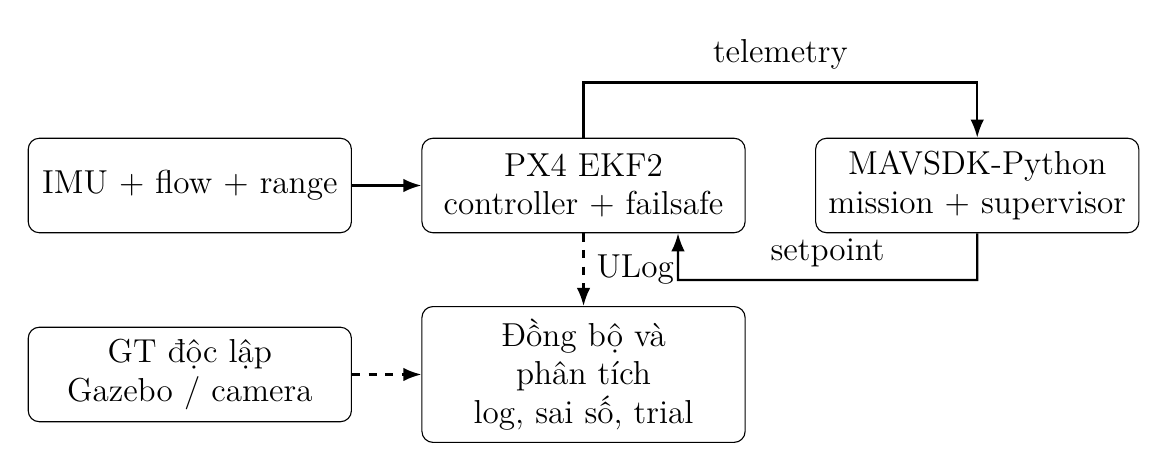
\begin{tikzpicture}[font=\fontsize{12}{14}\selectfont,box/.style={draw,rounded corners,align=center,text width=3.8cm,minimum height=1.2cm},arr/.style={-{Latex[length=2.3mm]},thick}]
\node[box] (s) at (0,0) {IMU + flow + range};
\node[box] (p) at (5,0) {PX4 EKF2\\controller + failsafe};
\node[box] (m) at (10,0) {MAVSDK-Python\\mission + supervisor};
\node[box] (g) at (0,-2.4) {GT độc lập\\Gazebo / camera};
\node[box] (a) at (5,-2.4) {Đồng bộ và phân tích\\log, sai số, trial};
\draw[arr] (s) -- (p);
\draw[arr] (p.north) -- ++(0,0.7) -| node[pos=0.25,above]{telemetry} (m.north);
\draw[arr] (m.south) -- (10,-1.2) -- node[above]{setpoint} (6.2,-1.2) -- ([xshift=1.2cm]p.south);
\draw[arr,dashed] (g) -- (a);
\draw[arr,dashed] (p) -- node[right]{ULog} (a);
\end{tikzpicture}
\captionof{figure}{Kiến trúc đề xuất: GT không đưa vào EKF2 hoặc vòng điều khiển.}\label{fig:architecture}
\end{center}

\subsection{Module giám sát chất lượng dữ liệu ở tầng nhiệm vụ}
Nhóm đề xuất điều phối điểm đặt theo trạng thái dữ liệu, không sửa estimator trong baseline đầu tiên. Khi local estimate hợp lệ và dữ liệu đạt yêu cầu, nhiệm vụ chạy bình thường; khi chất lượng suy giảm nhưng estimate vẫn dùng được, giới hạn tốc độ hoặc ngừng tiến waypoint; khi estimate mất hợp lệ, kích hoạt nhánh dừng nhiệm vụ và phản ứng an toàn đã kiểm chứng. Không coi lệnh giữ một vị trí local đã trôi là phương án an toàn trong mọi trường hợp.

Ngưỡng quality, tuổi dữ liệu và thời gian xác nhận trạng thái được chọn từ log hiệu chuẩn, có hysteresis hoặc dwell time để tránh chuyển trạng thái liên tục. Giá trị số chưa được đặt trong M1 vì chưa có dữ liệu đo. Nếu MAVSDK telemetry không cung cấp đủ health/quality, nhóm sẽ xác minh kênh MAVLink/ULog phù hợp trước khi cam kết module; không tự coi mọi trường EKF có sẵn qua API high-level.

Đóng góp cần kiểm chứng là \textbf{cách điều phối nhiệm vụ và phản ứng suy giảm dữ liệu} trên cấu hình N01. Không tuyên bố tính mới ở cấp công bố khoa học hoặc cải thiện estimator chỉ vì drone được yêu cầu bay chậm hơn. Nếu GVHD yêu cầu đóng góp trực tiếp ở estimator, nhóm cần điều chỉnh phạm vi và protocol trước khi sửa firmware.

\section{Kế hoạch kiểm chứng và tiêu chí đánh giá}
\subsection{Baseline, đối chứng và dữ liệu}
Baseline B0 dùng cùng PX4, tham số, model/world và chương trình waypoint tốc độ cố định, chưa bật supervisor bổ sung. Phương án B1 giữ nguyên nền đó và bật supervisor. Cùng kịch bản và điều kiện đầu, log được giữ cả lần đạt, lỗi và abort; không chọn một trial tốt để đại diện cả hệ. Nhóm lưu firmware commit, params, model/world, phiên bản phần mềm, seed nếu có, điều kiện sensor và đường dẫn log/GT/video.

Dữ liệu GT không dùng feedback trong B0/B1. Trước khi tính sai số, nhóm kiểm phép đổi ENU/NED, yaw/frame, gốc tọa độ, mốc thời gian và mẫu thiếu. Một kết quả chỉ có điểm đầu/cuối không đủ chứng minh sai số cực đại liên tục trong cửa sổ 30 s.

\subsection{Tách sai số giữ vị trí và sai số estimator}
Gọi $p_{sp}$ là vị trí đặt, $\hat p$ là vị trí ước lượng và $p_{GT}$ là vị trí đo độc lập sau đồng bộ. Nhóm đề xuất hai đại lượng ngang:
\begin{align}
e_{hold}(t)&=\|p_{GT,xy}(t)-p_{sp,xy}(t)\|_2,\\
e_{est}(t)&=\|\hat p_{xy}(t)-p_{GT,xy}(t)\|_2.
\end{align}
$e_{hold}$ đánh giá giữ vị trí của cả hệ; $e_{est}$ đánh giá estimator. Cách diễn giải đề xuất là kiểm $\max e_{hold}\leq0{,}5$ m trong cửa sổ 30 s và báo kèm max theo từng trục, RMSE, P95. Cách hiểu bán kính hay từng trục, số trial và cửa sổ nghiệm thu vẫn cần GVHD xác nhận; các metric phụ không thay KPI gốc~\cite{source1}.

Đối với square 2×2 m, nhóm báo sai số tại đỉnh, lệch cạnh, thời gian hoàn thành và tỷ lệ hoàn thành. Khi so B0/B1, phải báo thời gian và số abort để tránh kết luận phương án tốt hơn chỉ vì nó không di chuyển hoặc dừng quá nhiều.

\subsection{Kịch bản thử và giới hạn an toàn}
Bảng~\ref{tab:tests} là \textbf{kế hoạch thử}, không phải bảng kết quả. Tạo lỗi chỉ thực hiện trong SITL hoặc replay, không tạo lỗi khi bay thật.

\begingroup\tblfont
\begin{table}[ht]
\centering
\caption{Kịch bản kiểm chứng đề xuất}\label{tab:tests}
\begin{tabularx}{\linewidth}{L{3.0cm}YY}
\toprule Kịch bản & Quan sát bắt buộc & Tiêu chí/metric\\\midrule
Nominal hover & GPS fusion tắt; flow/range active; local valid; GT liên tục & Cửa sổ 30 s ở 1,0 và 1,5 m; max, RMSE, P95\\
Square 2×2 m & Setpoint, estimate và GT cùng frame/time & Sai số đỉnh/cạnh; thời gian; tỷ lệ hoàn thành\\
Flow/range suy giảm & Kịch bản có cách tạo lỗi được mô tả; health, quality, tuổi đo & Thời gian phản ứng; sai số GT; false-abort\\
Mất link/Offboard & Setpoint stream, trạng thái PX4, mất và phục hồi link & Phản ứng firmware và supervisor; lý do abort\\
Đối chứng B0/B1 & Cùng điều kiện, version và protocol & Trade-off sai số, thời gian và số lần dừng\\\bottomrule
\end{tabularx}
\end{table}
\endgroup

Mô hình flow của simulator có thể không tái hiện đầy đủ ánh sáng và texture thật. Trước khi dùng kịch bản thiếu sáng/sàn trơn, nhóm phải kiểm cách sensor được mô phỏng; nếu cần fault injection thì công bố rõ nó là lỗi đưa vào dữ liệu, không nhận là mô phỏng camera quang học hoàn chỉnh.

Thứ tự kiểm chứng bắt buộc: \textbf{G1 SITL; G2 bench không cánh; G3 hover thấp có bảo hộ; G4 square thật}. Bench kiểm nguồn, pinout, chiều/dấu cảm biến, range, RC takeover, kill và motor mapping. Bay thật chỉ khi có pilot/observer đủ năng lực, lưới/bảo hộ và vùng bay lớn hơn quỹ đạo để có biên drift/dừng. Không bỏ prearm checks hoặc mặc định RTL trong nhà. SITL không thay yêu cầu thử hover thật; thiếu điều kiện thì báo GVHD~\cite{source1}.

\section{Tiến độ, phân công đề xuất và việc đến M2}
Nhóm đã có đặc tả M0, kiến trúc và khảo sát sơ bộ; kiểm Drive ngày 10/10 xác nhận bản M0 có trong thư mục nhận bài từ 04/10, trước hạn. Chưa thấy file nhận xét trong thư mục nhận xét tại thời điểm kiểm. Báo cáo M1 này không nhận đã được thầy phê duyệt stack, KPI hoặc module.

Bảng~\ref{tab:next} nêu công việc và đầu ra để chuyển từ khảo sát sang module chạy được. \textbf{Phân công vẫn là phương án đề xuất, chưa xác nhận hai thành viên đã chốt}; nếu điều chỉnh, nhóm cập nhật trước khi cam kết tiến độ triển khai.

\begingroup\tblfont
\begin{table}[ht]
\centering
\caption{Kế hoạch sau M1 đến M2, hạn 09/11/2026}\label{tab:next}
\begin{tabularx}{\linewidth}{L{2.0cm}YYL{3.1cm}}
\toprule Mốc & Kiên (đề xuất) & Khanh (đề xuất) & Đầu ra\\\midrule
W03, đến 18/10 & Rà nguồn và lựa chọn, chốt phiên bản với N02 & Rà sensor/GT, thống nhất phân công & M1 PDF, danh sách quyết định mở\\
W04, 19--25/10 & Dựng baseline PX4 không GPS & Xuất GT, đồng bộ frame/time & Log đầu tiên, manifest; chưa đạt thì ghi blocker\\
W05, 26/10--01/11 & Mission local và supervisor tối thiểu & Script metric, kịch bản lỗi SITL & Module và check chạy được\\
W06, 02--08/11 & Tích hợp, luận giải, tài liệu chạy & Chạy thử, lưu trial, video & M2: PDF, Git, video 1--3 phút\\\bottomrule
\end{tabularx}
\end{table}
\endgroup

Các điểm cần xác nhận gồm: phạm vi đóng góp mission/safety hay estimator; cách đo KPI; release/commit và giao diện bàn giao N02; thiết bị Lab và khu bay. Nếu chưa có môi trường N02, nhóm đề xuất baseline tối thiểu khóa phiên bản, ghi rõ khác biệt để không phụ thuộc hoàn toàn ngày bàn giao. Không dựng hai stack đồng thời.

\section{Kết luận}
Khảo sát cho thấy OF kết hợp range và IMU có cơ sở triển khai giữ vị trí không GPS, nhưng số liệu từ các công trình khác cấu hình không chứng minh KPI N01. Nhóm lựa chọn PX4 EKF2 làm nền đề xuất vì phù hợp cảm biến, có controller/fusion và thuận lợi phối hợp N02; ArduPilot là phương án dự phòng hợp lệ, VIO/observer mới chưa phù hợp phạm vi hiện tại.

Phần tiếp theo là kiểm baseline bằng log và GT độc lập, sau đó đối chứng supervisor ở tầng nhiệm vụ. Tại thời điểm báo cáo, nhóm chưa có bằng chứng SITL/bench/flight pass. Lợi ích của module vẫn là giả thuyết cần kiểm chứng; kết quả không cải thiện cũng sẽ được lưu và phân tích.

\begingroup\setstretch{1.0}\normalsize\raggedright
\begin{thebibliography}{99}
\bibitem{source1} N. D. X. Bách, “Đồ án 1 -- Đồ án 2, HK1 2026--2027: Mô tả đề tài và kế hoạch thực hiện,” Khoa KTMT, UIT, email 25/09/2026, tr. 1--2, 4, 12. Tài liệu GVHD cung cấp.
\bibitem{source2} PX4 Development Team, “Optical Flow,” \textit{PX4 User Guide}, bản nguồn lưu 29/09/2026. [Online]. Available: \url{https://docs.px4.io/main/en/sensor/optical_flow.html}.
\bibitem{source3} PX4 Development Team, “Using PX4's Navigation Filter (EKF2),” \textit{PX4 User Guide}, bản nguồn lưu 29/09/2026. [Online]. Available: \url{https://docs.px4.io/main/en/advanced_config/tuning_the_ecl_ekf.html}.
\bibitem{source4} N. Gageik, M. Strohmeier, and S. Montenegro, “An autonomous UAV with an optical flow sensor for positioning and navigation,” \textit{Int. J. Adv. Robot. Syst.}, vol. 10, no. 10, 2013, doi: \href{https://doi.org/10.5772/56813}{10.5772/56813}.
\bibitem{source5} R. Wang, D. Zou, C. Xu, L. Pei, P. Liu, and W. Yu, “An aerodynamic model-aided state estimator for multi-rotor UAVs,” in \textit{Proc. IEEE/RSJ IROS}, 2017, pp. 2164--2170, doi: \href{https://doi.org/10.1109/IROS.2017.8206034}{10.1109/IROS.2017.8206034}.
\bibitem{source6} V. Grabe, H. H. Bülthoff, D. Scaramuzza, and P. R. Giordano, “Nonlinear ego-motion estimation from optical flow for online control of a quadrotor UAV,” \textit{Int. J. Robot. Res.}, vol. 34, no. 8, pp. 1114--1135, 2015, doi: \href{https://doi.org/10.1177/0278364915578646}{10.1177/0278364915578646}.
\bibitem{source7} M.-T. Nguyen \textit{et al.}, “Stabilzation position of quadcopter using vision-based corner detector from top-down footage of camera,” \textit{J. Tech. Educ. Sci.}, no. 71A, pp. 18--27, 2022, doi: \href{https://doi.org/10.54644/jte.71A.2022.1132}{10.54644/jte.71A.2022.1132}.
\bibitem{source8} J. R. Meza-Ibarra, J. Martínez-Ulloa, L. A. Moreno-Pacheco, and H. Rodríguez-Cortés, “A sensor fusion approach to observe quadrotor velocity,” \textit{Sensors}, vol. 24, no. 11, art. 3605, 2024, doi: \href{https://doi.org/10.3390/s24113605}{10.3390/s24113605}.
\bibitem{source9} T. Qin, P. Li, and S. Shen, “VINS-Mono: A robust and versatile monocular visual-inertial state estimator,” arXiv:1708.03852, 2017; bản tạp chí \textit{IEEE Trans. Robot.}, 2018, doi: \href{https://doi.org/10.1109/TRO.2018.2853729}{10.1109/TRO.2018.2853729}. Tóm tắt đối chiếu ngày 10/10/2026: \url{https://arxiv.org/abs/1708.03852}.
\bibitem{source10} PX4 Development Team, “ARK Flow,” \textit{PX4 User Guide}, bản nguồn lưu 29/09/2026. [Online]. Available: \url{https://docs.px4.io/main/en/dronecan/ark_flow.html}.
\bibitem{source11} ArduPilot Development Team, “Optical flow sensor testing and setup,” \textit{Copter Documentation}, truy cập 10/10/2026. [Online]. Available: \url{https://ardupilot.org/copter/docs/common-optical-flow-sensor-setup.html}.
\bibitem{source12} PX4 Development Team, “Gazebo Simulation,” \textit{PX4 User Guide}, bản nguồn lưu 29/09/2026. [Online]. Available: \url{https://docs.px4.io/main/en/sim_gazebo_gz/}.
\bibitem{source13} PX4 Development Team, “Offboard Mode,” \textit{PX4 User Guide}, bản nguồn lưu 29/09/2026. [Online]. Available: \url{https://docs.px4.io/main/en/flight_modes/offboard.html}.
\end{thebibliography}
\endgroup
\end{document}
